\section{Analysis}
%\FloatBarrier % Now figures cannot float above section title
Next the experimental data were processed. Firstly the difference in water head was calculated for each sampling point on tapping position by using the Pitot tube at atmospheric pressure as a standard value. The difference in water head was then converted to a difference in pressure by equation $P_n=\rho gh$, as shown in \autoref{t5.1} below.
% Please add the following required packages to your document preamble:
% \usepackage{booktabs}
\begin{table}[htbp]
    \caption{Preliminary processing of experimental data (Unit: Pa)} 
	\label{t5.1}
    \resizebox{1\textwidth}{!}{
    \begin{tabular}{@{}cccccccccccccccc@{}}\toprule
    Degree/Pitot No.   & 1      & 3       & 5       & 7       & 9       & 11     & 2        & 4        & 6       & 8       & 10      & 12      & Atm & Airbox & Inlet  \\\midrule
    0$^\circ$    & 98.1   & -274.68 & -333.54 & -274.68 & -186.39 & -88.29 & -19.62   & -294.3   & -304.11 & -215.82 & -156.96 & -39.24  & 0   & 568.98 & 39.24  \\
    5$^\circ$    & 490.5  & 88.29   & -107.91 & -107.91 & -78.48  & -39.24 & -608.22  & -667.08  & -529.74 & -372.78 & -176.58 & -58.86  & 0   & 568.98 & 58.86  \\
    10$^\circ$   & -392.4 & 333.54  & 107.91  & 9.81    & 19.62   & 9.81   & -1255.68 & -961.38  & -784.8  & -392.4  & -215.82 & -58.86  & 0   & 568.98 & 78.48  \\
    15$^\circ$   & 568.98 & 480.69  & 255.06  & 127.53  & 78.48   & 29.43  & -1697.13 & -1294.92 & -686.7  & -392.4  & -196.2  & -78.48  & 0   & 568.98 & 117.72 \\
    17.5$^\circ$ & 549.36 & 519.93  & 304.11  & 166.77  & 98.1    & 39.24  & -1746.18 & -1412.64 & -657.27 & -372.78 & -206.01 & -78.48  & 0   & 568.98 & 137.34 \\
    20$^\circ$   & 598.41 & 490.5   & 304.11  & 186.39  & 107.91  & 39.24  & -294.3   & -313.92  & -313.92 & -323.73 & -313.92 & -274.68 & 0   & 568.98 & 235.44 \\
    22.5$^\circ$ & 608.22 & 510.12  & 333.54  & 225.63  & 137.34  & 58.86  & -215.82  & -235.44  & -235.44 & -255.06 & -255.06 & -235.44 & 0   & 568.98 & 274.68 \\
    25$^\circ$   & 598.41 & 549.36  & 392.4   & 304.11  & 186.39  & 98.1   & -137.34  & -156.96  & -166.77 & -176.58 & -215.82 & -215.82 & 0   & 588.6  & 313.92 \\ \bottomrule
    \end{tabular}}
    \end{table}




Based on the \autoref{t5.1}, it was able to calculate the effective static pressure ($p_{eff}$) in different angle by given \autoref{Peff}.
\begin{equation}
    \label{Peff}
   p_{eff}=p_{0}+\frac{85}{135}\times(p_{a}-p_{0})
    \end{equation}
($P_0$ is the inlet pressure)
And calculate free stream velocity $U_\infty$ by given \autoref{Uinf} in different angle.
\begin{equation}
    \label{Uinf}
    U_{\infty}={\sqrt{\frac{2\times(p_{airbox}-p_{eff})}{\rho}}}
    \end{equation}
The results are shown in the following \autoref{t5.2}.
% Please add the following required packages to your document preamble:
% \usepackage{booktabs}
And from \autoref{cpn},
\begin{equation}
    \label{cpn}
    C_{p,n}={\frac{p_n-p_{eff}}{{\frac{1}{2}}\rho u_{\infty}^{2}}}
    \end{equation}
the pressure ratio in different angle can be calculated. Additionally, the tapping position and aerofoil chord for the different sampling points can be obtained from the appendix which is in handbook, and the $x/c$ can be calculated. The initial and final points of the curves (0, 0) and (1, 0) have been added to the figures according to the lab handbook. The images are connected by using a smooth curve (Piecewise Cubic Hermite Interpolating Polynomial) as shown in \autoref{t5.3}.\footnote{Regression analysis is not applicable to smooth curve fitting.}
\begin{table}[htbp]
    \caption{$p_{eff}$ and $U_\infty$ in different angle (Unit: Pa and m/s)} 
	\label{t5.2}
    \resizebox{1\textwidth}{!}{
    \begin{tabular}{@{}ccccccccc@{}}\toprule
      Pitot No.   & 0        & 5        & 10       & 15       & 17.5     & 20       & 22.5     & 25       \\\midrule
    $p_eff$ & 24.70667 & 37.06    & 49.41333 & 74.12    & 86.47333 & 148.24   & 172.9467 & 197.6533 \\
    $U_\infty$ & 30.11847 & 29.77471 & 29.42693 & 28.71875 & 28.35803 & 26.48081 & 25.69155 & 25.52602\\\bottomrule
    \end{tabular}}
    \end{table}
\begin{table}[htbp]
    \caption{Pressure ratio ($C_p$) in different angle and degree} 
	\label{t5.3}
    \resizebox{1\textwidth}{!}{
    \begin{tabular}{@{}ccccccccccccc@{}}\toprule
    Pitot No.     & 1      & 3      & 5      & 7      & 9      & 11     & 2      & 4      & 6      & 8      & 10     & 12     \\
    $x/c$     & 0.016  & 0.071  & 0.175  & 0.317  & 0.510  & 0.698  & 0.032  & 0.119  & 0.230  & 0.413  & 0.603  & 0.794  \\\midrule
    0    & 0.135  & -0.560 & -0.613 & -0.505 & -0.342 & -0.162 & -0.036 & -0.541 & -0.559 & -0.397 & -0.288 & -0.072 \\
    5    & 0.852  & 0.110  & -0.203 & -0.203 & -0.148 & -0.074 & -1.143 & -1.254 & -0.996 & -0.701 & -0.332 & -0.111 \\
    10   & -0.850 & 0.585  & 0.208  & 0.019  & 0.038  & 0.019  & -2.417 & -1.850 & -1.510 & -0.755 & -0.415 & -0.113 \\
    15   & 1.000  & 0.913  & 0.515  & 0.258  & 0.159  & 0.059  & -3.430 & -2.617 & -1.388 & -0.793 & -0.396 & -0.159 \\
    17.5 & 0.959  & 1.019  & 0.630  & 0.346  & 0.203  & 0.081  & -3.619 & -2.928 & -1.362 & -0.773 & -0.427 & -0.163 \\
    20   & 1.070  & 1.103  & 0.723  & 0.443  & 0.256  & 0.093  & -0.699 & -0.746 & -0.746 & -0.769 & -0.746 & -0.653 \\
    22.5 & 1.099  & 1.223  & 0.842  & 0.570  & 0.347  & 0.149  & -0.545 & -0.594 & -0.594 & -0.644 & -0.644 & -0.594 \\
    25   & 1.025  & 1.340  & 1.004  & 0.778  & 0.477  & 0.251  & -0.351 & -0.401 & -0.427 & -0.452 & -0.552 & -0.552\\\bottomrule
    \end{tabular}}
    \end{table}

Based on \autoref{t5.3}, Pressure distributions are plotted as a graph of the pressure ratio, which at 8 different angles with $x/c$ as the x-axis and $C_p$ as the y-axis. The figure is shown in \autoref{cp}.
\begin{figure}[htbp]
    \centering
    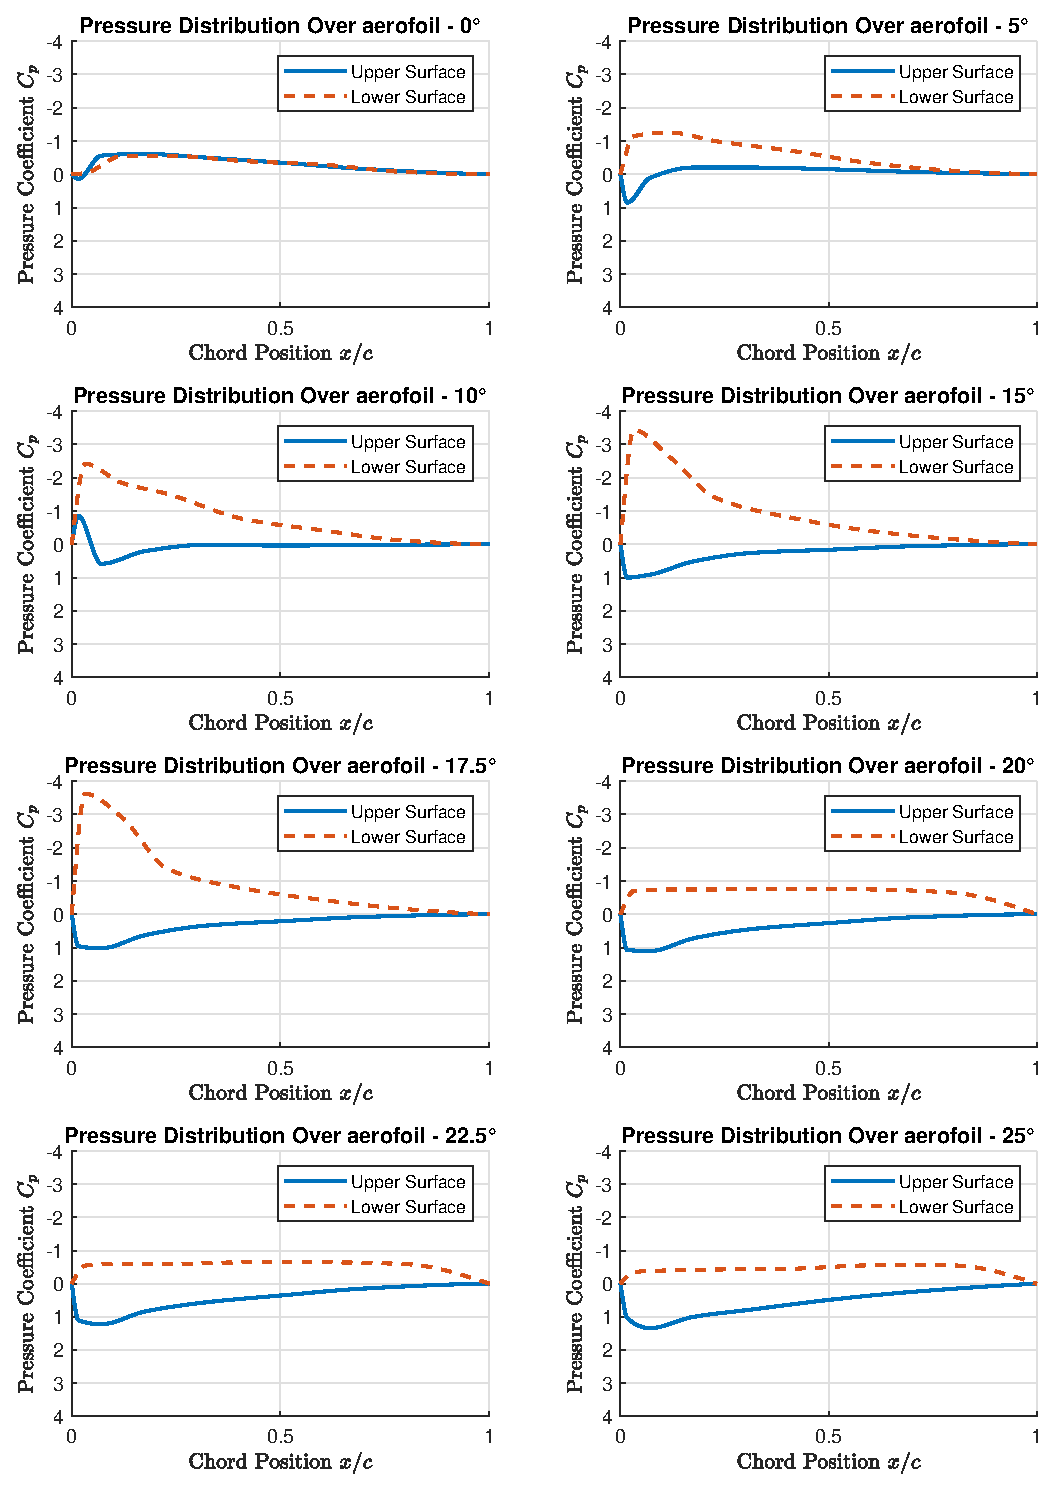
\includegraphics[width=0.92\textwidth]{output.eps}
    \caption{Pressure distribution over aerofoil}
    \label{cp}
  \end{figure}
By using the \autoref{cl}, We can calculate lift coefficient $C_L$.
\begin{equation}
    \label{cl}
C_{L}={\frac{F_{L}}{{\frac{1}{2}}\rho U^{2}A}}
\end{equation}
Noticed that A is the plan area of the aerofoil. By using mathematical method, this can be evaluated by given equation:
$$
C_{L}=\int\left[C_{p l}\left(\frac{x}{c}\right)-C_{p u}\left(\frac{x}{c}\right)\right]d\left(\frac{x}{c}\right)
$$
However, an important point to note is that a direct integration requires a continuous function. In order to find the solution, we use discrete data points to evaluate the $C_L$ by using trapezoidal rule. So, the discrete version of the integral becomes:
$$
\Delta C_{L}=\sum\left(\frac{C_{pl,i+1}+C_{pl,i}}{2}-\frac{C_{p u ,i+1}+C_{p u ,i}}{2}\right)\left(x_{i+1}-x_{i}\right)
$$
Where $i$ is the index of the data points. The results show in \autoref{t5.4} and \autoref{tcl}.
\begin{table}[]
    \caption{Lift coefficient ($C_L$) in different angle} 
	\label{t5.4}
    \centering
    \resizebox{0.8\textwidth}{!}{
    \begin{tabular}{@{}ccccccccc@{}}\toprule
     Degree    & 0        & 5        & 10       & 15       & 17.5     & 20       & 22.5     & 25       \\\midrule
    $C_L$ & -0.040 & 0.383 & 0.676 & 0.939 & 1.015 & 0.840 & 0.828 & 0.830\\\bottomrule
    \end{tabular}}
    \end{table}

\begin{figure}[htb] % Here, top, bottom priority list
        \centering
        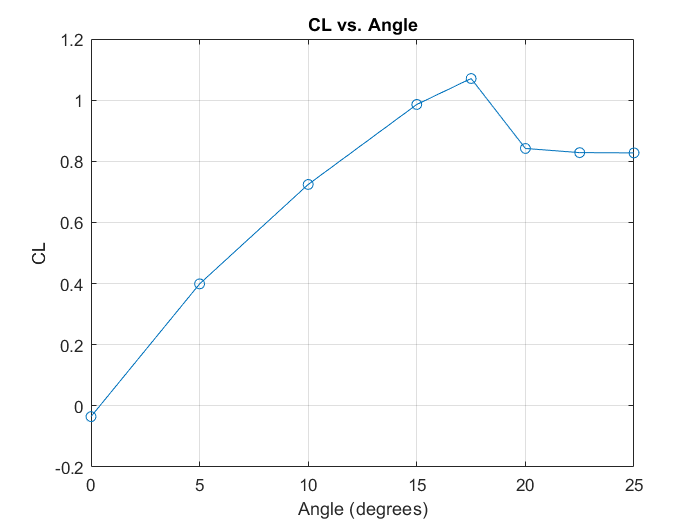
\includegraphics[scale=0.5]{CL.eps}
        \caption{$C_L$ vs Angle}
        \label{tcl}
\end{figure}
